%
% Fachseminararbeit · Wintersemester 2011/2012 Fachbereich Design Informatik Medien · Hochschule RheinMain Bachelor-Studiengang Medieninformatik
%
% Thema: Dynamische Integration von Webservices
% Untertitel: Konzepte und Standards zur domänenübergreifenden Integration von komplexen Webanwendungen
%
% @author: Markus Tacker <m@coderbyheart.de>
% @link https://github.com/tacker/fachseminar/
% 
\documentclass[10pt,a4paper]{article}
\usepackage[utf8]{inputenc}
\usepackage[german]{babel}
\usepackage[T1]{fontenc}
\usepackage{graphicx}

\usepackage[paper=a4paper,width=14cm,left=35mm,height=22cm]{geometry}
\usepackage{setspace}
\usepackage{acronym}
\usepackage{charter}

\usepackage{color}
\usepackage{listings}
\lstset{
	basicstyle=\sffamily, 
	columns=[l]flexible, 
	mathescape=true, 
  	showstringspaces=false, 
  	numbers=left, 
  	numberstyle=\tiny,
  	keywordstyle=\color[rgb]{0,0,1},
    commentstyle=\color[rgb]{0.133,0.545,0.133},
    stringstyle=\color[rgb]{0.627,0.126,0.941},
}
\lstset{language=xml}
\usepackage{float}
\newfloat{listing}{htbp}{scl}[section]
\floatname{listing}{Listing}

\linespread{1.15}
\setlength{\parskip}{0.5em}
\setlength{\parindent}{0em}

\bibliographystyle{plain} 
\bibdata{bibliothek}

\usepackage[usenames,dvipsnames]{xcolor}
\usepackage{hyperref}
\hypersetup{
    bookmarks=true,
    colorlinks=true,
    linkcolor=NavyBlue,
    citecolor=NavyBlue,
    urlcolor=NavyBlue
}

% Abkürzungen werden hier definiert, da es kein "öffentliches" Abkürzungsverzeichnis gibt

\newacro{SOAP}[SOAP]{Simple Object Access Protocol}
\newacro{UDDI}[UDDI]{Universal Description, Discovery and Integration}
\newacro{ORISF}[ORISF]{Ontology-based Resourceoriented Information Supported Framework}
\newacro{WSDL}[WSDL]{Web Services Description Language}
\newacro{SAWSDL}[SAWSDL]{Semantic Annotations for WSDL}
\newacro{SOA}[SOA]{Service Oriented Architecture}
\newacro{API}[API]{Application Programming Interface}
\newacro{mite}[\emph{mite}]{\emph{mite}\footnote{http://mite.yo.lk/}}

\begin{document}
\author{Markus Tacker}
\title{Dynamische Integration von Webservices}

\begin{center}

\begin{small}Fachseminararbeit · Wintersemester 2011/2012\\\href{http://www.hs-rm.de/dcsm}{Fachbereich Design Informatik Medien} · \href{http://www.hs-rm.de/}{Hochschule RheinMain}\\\href{http://www.hs-rm.de/medieninformatik}{Bachelor-Studiengang Medieninformatik}\end{small}

\bigskip

\begin{huge}Dynamische Integration von Webservices\end{huge}

\begin{small}Konzepte und Standards zur domänenübergreifenden\\Integration von komplexen Webanwendungen\end{small}

\bigskip

\begin{large}\href{http://markusstudiert.de/}{Markus Tacker}\end{large}

\begin{small}\url{https://github.com/tacker/fachseminar/}\end{small}

\today

\end{center}

\section*{Abstract}

Die Integration von Webservices erfolgt in der Regel durch das Entwickeln von Adaptern in der Umgebung, in der die Integration erfolgen soll. In dieser Fachseminararbeit stelle ich Standards und Konzepte vor, die diesen Vorgang weitestgehend automatisieren können. Voraussetzung dafür ist, dass Webservices semantisch beschrieben werden, erst dann ist eine automatische Dienstvermittlung zur Laufzeit möglich. Wie Dostal und Jeckle aber in \cite[S.55]{xmlspek1} beschreiben, wurden jedoch Standards zur Anbindung von Webservices wie z.B. \acs{WSDL} im Hinblick auf die Anbindung von \emph{Services} mit einer konkreten \acs{API} entwickelt --- sie beschreiben den syntaktischen Rahmen einer Schnittstelle, das zu Grunde liegende Wissen über das Domänenkonzept, also die \emph{Semantik}, wird nicht beschrieben. Nach einer Einführung in das Thema in Abschnitt~\ref{l:einleitung}, in dem der aktuelle Stand der Entwicklung beschrieben wird und die daraus resultierende Hindernisse bei der dynamischen Bindung von Webservice erläutert werden, führt Abschnitt~\ref{l:sem-web-ser} in die theoretischen Aspekte ein und zeigt wie man mit Hilfe von \emph{Ontologien} Domänenkonzepte semantisch beschreibbar machen kann. Mit der \acs{SAWSDL} existiert ein Standards für diese Aufgabe, der in Abschnittes~\ref{l:sawsdl} beschrieben wird. Abschnitt~\ref{l:loesungen} stellt mögliche Lösungsansätze für die Implentierung einer \acs{SOA} vor, deren Dienste zur Laufzeit gebunden werden. Im Fazit in Abschnitt~\ref{l:fazit} werden die aufgezeigten Konzepte auf ihre Anwendbarkeit auf \emph{komplexen Webanwendungen} analysiert.

\section{Einleitung}
\label{l:einleitung}
\section{Einleitung}
\label{l:einleitung}

Ein Teil der neueren Entwicklung des Internets zum \emph{Web 2.0} basiert auf der Idee, dass Informationen und Funktionen von Software mit Hilfe von \emph{Webservices} verwendet werden können.

Die Kommunikation mit Webservices ist zwar auf Protokollebene standardisiert, muss jedoch vom Konsumenten immer individuell entsprechend dem Domänenmodell des Anbieters implementiert werden, wodurch eine feste Bindung an den Anbieter entsteht. \cite{ka-cots}

Für sogenannte \emph{Blackbox-Webservices} ist das kein Problem --- diese zustandslose Dienste verarbeiten lediglich einfache Daten, d.h. dass der Dienst durch Übergabe eines Datums aufgerufen wird, dieser entsprechend des Aufrufs reagiert und ein Ergebnis zurück liefert.

Diese Eigenschaft steht in direktem Zusammenhang mit einem wichtigen Trend in der Softwareentwicklung: \ac{SOA} bei der Anwendungen nicht mehr monolitisch aufgebaut werden, sondern sich in kleiner, in sich geschlossene Komponenten unterteilt, die miteinander über netzwerkbasierte, öffentliche Schnittstellen, die sogenannte \ac{API}, kommunizieren.

Diese Kapselung von Diensten hat auch zum Ziel, eine möglichst hohe Kohäsion innerhalb eines Systems zu ermöglichen --- Code soll wenn möglich nur einmal geschrieben werden, und im ganzen System verwendet werden können, woraus im Endergebnis weniger Code, niedrigere Kosten und eine höhere Standardisierung resultieren. \cite{hn-web20}

% MARK

Anbieter \emph{webbasierter Anwendungen} stehen jedoch vor dem Problem, dass auf Seiten des Anbieters komplexe Arbeitsabläufe abgebildet werden und diese auch persistent innerhalb des Dienstes verbleiben, d.h. sie sind zustandsbehaftet. Auch hier bietet sich die Möglichkeit der Anbindung mittels Schnittstellen, jedoch mit deutlich gesteigertem Aufwand, da zwischen beiden Parteien das Verständnis über die verarbeiteten 
Entitäten vermittelt werden muss. 

Nach \cite[Seite 653]{ei-sawsdl} sind etablierte Standards für Webservices der ersten Generation wie \ac{SOAP} und \ac{UDDI} primär unter dem Aspekt entwickelt worden, einen einfachen Weg zur Verteilung und Wiederverwertung von Webservices zu etablieren --- ihnen fehlt also eine Standardisierung für das Auffinden, Zusammenstellen und Auswählen von Diensten um eine \emph{lose Kopplung} zu ermöglichen. Für ein lebendiges Web-Öko-System ist die lose Kopplung jedoch von entscheidender Bedeutung --- im Idealfall lassen sich Dienste so anbinden, dass sie jederzeit und ohne Aufwand ausgetauscht werden können und sogar die parallele Verwendung mehrere Dienste der gleichen Art ermöglicht wird.  

% Infos zu Blackbox-WS einfließen lassen

Für die Nutzung eines Dienstes reicht die Kenntnis der Schnittstellen aus. Ein tieferes Verständnis der internen Vorgänge wird nicht benötigt, bzw. soll bewusst verborgen werden. \cite{hhxmlwssoa}

Beispiele hierfür ist z.B. ein Webservice, der Wetterdaten für eine PLZ liefert. Hier gibt der Konsument die PLZ eines Ortes in Deutschland ein und erhält in der Antwort eine Temperatur. Die genauen technischen Abläufe, wie der Webservice aus der PLZ eine Temperatur ermittelt bleiben für den Konsumenten verborgen und sind für diesen auch irrelevant.

Diese Arten von Diensten sind zustandslos, d.h. sie behandlen jede Anfrage unabhängig von einer vorherigen.

% Infos zu Whitebox-WS einfließen lassen
% Webbasierte Anwendungen, Whitebox-Dienste

Nicht zustandslos.

Beispiele hierfür sind z.B. Werkzeuge zur projektspezifischen Zeiterfassung. 

% Beispiele einfließen lassen

\begin{itemize}
\item Mite
\item E-Mail-Backup
\end{itemize}

% Hinweis auf Ökonomische Aspekte, Ultra Large Scale Systems

Eine Möglichkeit die Überlebensfähigkeit von digitalen Ökosystemen sicherzustellen ist es, Redundanz einzuführen und zwar Redundanz auf allen Ebenen, angefangen von der Hardware über die Betriebssysteme bis hin zur Software und den eingesetzten Services. Ein solch hohes Maß an Redundanz würde jedoch immense Investitionen verschlingen, von daher ist es günstiger, mit einer minimalen Redundanz zu leben und die Qualitäten der gelieferten Services zu reduzieren. Für die Qualitätsreduktion ist jedoch wichtig zu wissen, was an Services vom System noch in welcher Qualität zur Verfügung steht und was nicht. Die "überlebenden" Services werden neu komponiert und den Consumern zur Verfügung gestellt. Diese Form der ad-hoc Komposition bedingt, dass Servicekomposition (s. Abschn. 2.7.3) sich neben den fachlichen Interfaces und den "bestmöglichen" Qualitäten auch an Notfallpolicies orientieren kann. \cite{mkulss}


\section{Semantische Webservices}
\label{l:sem-web-ser}
Wie im vorigen Abschnitt beschrieben wurde, fehlt der bisherigen Beschreibung von Webservices der semantische Aspekt. Unter \emph{semantischen \acl{WS}} versteht man solche \acl{WS}, deren Beschreibung neben der konkreten technischen Aspekten zur Anbindung auch Information zur abgebildeten "`Welt"' enthalten. In diesem Abschnitt erläutere ich deren Grundlagen.

\subsection{Semantik}

Die \emph{Semantik} (griechisch, "`Bezeichnung"') beschreibt das Wesen von Dingen und ermöglicht die Interpretation und Übertragung von Konzepten auf konkrete Begebenheiten. Semantik ist die Grundlage jeglicher Kommunikation und umgibt uns überall. Bereits in jungen Jahren lernen wir, dass ein über einem Weg hängender Kasten, aus dem uns ein Licht rot anstrahlt eine \emph{bestimmte} Bedeutung hat. Nach einiger Zeit verbinden wir damit intuitiv: "`Halt, hier geht es nicht weiter."' Wichtig ist allerdings, dass die scheinbar eindeutige Verbindung zwischen der Farbe "`Rot"' und dem Konzept "`Nicht weiter gehen!"' kontextabhängig ist. Begegnet uns ein leuchtendes Rot auf einem Apfel, wissen wir, dass das Obst frisch und genießbar ist. Die Bedeutung "`Halt!"' der Farbe Rot verdreht sich in diesem Kontext in das Gegenteil: "`Iss mich!"'.

Wie schon auf Seite \pageref{l:intro-loosecoupling} beschrieben, ist Voraussetzung für eine Service-Infrastruktur mit loser Kopplung, dass die Bedeutung der Aufgabe, die mit dem Webservice abgebildet wird automatisch ermittelt werden kann.

Beschreibt man einen Webservice z.B. mittels der \ac{WSDL}, legt man damit lediglich den Syntax für die vom Webservice verarbeiteten Anfragen fest. Die Bedeutung der Funktionalität und der übertragenen Daten erschließt sich daraus nicht. Sie entsteht lediglich in der Interpretation der Benutzer des Dienstes. 

In Listing \ref{code:wsdl} auf Seite \pageref{code:wsdl} findet sich eine \ac{WSDL} für der Webservice "`PeopleAsk"'\footnote{http://peopleask.ooz.ie/}, mit dem sich die aktuell in Google gestellten Fragen abrufen lassen. Beschrieben werden die Entitäten \emph{GetQuestionsAbout} mit dem Attribut \emph{query} und \emph{GetQuestionsAboutResponse}, das eine Liste mit Strings ist. Aus dem Dokument geht jedoch nicht hervor, dass eigentlich \emph{Suchanfragen} einer \emph{Suchmaschine} zurückgegeben werden --- dieses Wissen entsteht aus Informationen, die nur außerhalb der Schnittstellenbeschreibung zugänglich sind.

Es fehlt also eine Komponente, die dem reinen Akt der Datenübertragung ein inhaltlichen Beschreibung, hinzufügt und das zudem noch in maschinenlesbarer Form. In der Informatik sind das \emph{Ontologien}.

Ontologien sind die \emph{Spezifikation eines Konzepts}. \emph{Spezifikation} bedeutet dabei eine formale und deklarative Repräsentation, die damit automatisch maschinenlesbar ist und Missverständnisse ausschließt. Ein \emph{Konzept} ist die abstrakte und vereinfachte Sicht der für das Konzept relevanten Umgebung. Ontologien beschreiben aus der Sicht des Dienstanbieters die Zusammenhänge in der Umgebung, auf die durch den Webservice implizit zugegriffen wird. In \cite[S.31]{dcswe} liefert Devedžić zum bessern Verständnis dieses Bildnis: Möchte eine Person über Dinge aus der Domäne \emph{D} mit der Sprache \emph{L} sprechen, beschreiben Ontologien die Dinge, von denen angenommen wird, dass sie in \emph{D} als Konzepte, Beziehungen und Eigenschaften von \emph{L} existieren.

\subsection{Semantische Beschreibung von \acl{WS}}\label{l:sawsdl}

Mit den \ac{SAWSDL} hat das \ac{W3C} 2007 einen Entwurf zu einem Standard vorgelegt, der es ermöglicht Informationen zu diesen Ontologien maschinenlesbar, als Teil einer \ac{WSDL}-Datei, auszuliefern. 

\ac{SAWSDL} ist dabei unabhängig von einem semantischen Konzept und liefert nur den Rahmen um andere semantische Frameworks in \ac{WSDL} zu integrieren --- es wird lediglich vorausgesetzt, dass diese Konzepte anhand von URIs identifierziert werden können \cite[S.61]{ky-sawsdl}. Eine Mögliche Technik zur semantischen Beschreibung ist, \ac{OWL}, das auf \ac{RDF} basiert. In \ac{RDF} werden dabei die Entitäten (in \ac{RDF} "`Ressourcen"' genannt) mit ihren Attributen und Beziehungen untereinander syntaktisch beschrieben \cite{w3c-rdf}. In \ac{RDF} fehlt aber die Möglichkeit, die Beziehungen von Eigenschaften zu beschreiben. Zum Beispiel besitzt ein Buch das Attribut \emph{Autor}. Dass damit aber eine weitere Ressource gemeint ist (eine \emph{Person} mit der Rolle \emph{Autor}) lässt sich in einem \ac{RDF}-Dokument nicht hinterlegen. Mit \ac{RDFS} wurde deswegen die Möglichkeit geschaffen, Gruppen zusammengehöriger Ressourcen und ihrer Beziehung untereinander zu beschreiben \cite{w3c-rdfs}. Mit \ac{OWL} ist es schließlich möglich, Ontologien in Form von Klassen, Eigenschaften, Instanzen und Operationen zu beschreiben \cite{w3c-owl2primer}.

In \ac{WSDL} werden \acl{WS} auf einer syntaktischen Ebene beschrieben. Es wird festgelegt, wie die auszutauschenden Nachrichten \emph{aussehen} und an welchen Endpunkten der \ac{API} diese zum Einsatz kommen, nicht jedoch was sie bedeuten. In \ac{WSDL} werden die abstrakten Elemente \emph{Element Declaration}, \emph{Type Definition} und \emph{Interface} verwendet, um einen Webservice allgemein zu beschreiben, hier spielen die technischen wie das verwendete Protokoll keine Rolle. Ein \emph{Type} entspricht dabei einem Objekt aus der Domäne, ein \emph{Element} beschreibt ein Attribut dieses Objekts. Ein \emph{Interface} beschreibt die Operationen und deren Parameter, die von der Schnittstelle unterstützt werden. In Listing \ref{code:wsdl2} auf Seite \pageref{code:wsdl2} findet sich ein einfaches Beispiel einer \ac{WSDL}-Datei.

\ac{SAWSDL} führt nun für diese drei Elemente zusätzlich Attribute ein, um deren semantische Bedeutung zu beschreiben:

\begin{itemize}
\item \texttt{modelReference} definiert eine Beziehung zwischen einem der definierten Komponente in der \ac{WSDL} und einem Objekt im semantischen Modell. Diese Attribut kann auf jedes \ac{WSDL}- oder XML-Schema-Element angewendet werden. Der Wert des Attributes ist dabei eine oder mehrere URIs, die auf ein semantisches Modell verweisen.
\item Die Attribute \texttt{liftingSchemaMapping} und \texttt{loweringSchemaMapping}, die auf Typedefinitionen definiert werden können, spezifizieren das Mapping zwischen semantischen Daten (z.B. \ac{RDF} und XML) sowie umgekehrt. Hierbei ist es auch möglich, mehrere Mappings je Typ zu definieren, um verschiedene Repräsentation je Kontext zu ermöglichen. Die \emph{lifting}- und \emph{lowering}-Transformationen sind nützlich, wenn von einem semantischen Client aus mit einem \acl{WS} kommunziert wird. Für eine Anfrage werden dann die Semantischen Daten in das Anfrage-Format des Client durch \emph{lowering} transformiert, die Antwort wird dann durch \emph{lifting} wieder in ein semantisches Format konvertiert.
\end{itemize}\cite[S.62ff]{ky-sawsdl}

% TODO: Abbildung 3 aus \cite{ky-sawsdl} rein

Dieses Verfahren kommt auch bei der Verwendung einer gemeinsamen Ontologie zum Einsatz --- ein automatischer Vermittler kann dabei die Daten zwischen zwei Schnittstellen mit den \emph{Lifting}-Informationen des Anfragers und den \emph{Lowering}-Informationen des Empfängers vermitteln.

% TODO: Abbildung 4 aus \cite{ky-sawsdl} rein

% TODO: http://www.docstoc.com/docs/82666005/SAWSDL-tutorial-at-Semantic-Technology-Conference-2007

% MARK

\begin{itemize}
\item http://www.w3.org/TR/sawsdl-guide/
\item \ac{SAWSDL} und \ac{REST}? \cite{xn-sss}
\item \ac{SAWSDL} verwenden: Grüner Kasten in \cite[S.63]{ky-sawsdl}, \cite{flexbrok} und sehr ausführlich in \cite{vr-sesa}
\end{itemize}

\section{Dynamische Verwendung von semantischen Webservices}
\label{l:loesungen}
\ac{RDF} als Möglichkeit, Semantik in XML zu beschreiben.

In this paper we will explore this issue in some detail and we will propose a set of
features that, in our view, will increasingly characterize the Semantic Web
applications. Our analysis aims to be both descriptive and prescriptive. Descriptively,
the objective here is to characterize the space of current Semantic Web applications,
provide dimensions to compare and contrast them, and identify key trends.
Prescriptively, our goal is to specify a number of criteria, which Semantic Web
applications ought to satisfy, if we want to move away from conventional semantic
systems and develop a new generation of Semantic Web applications, which can
succeed in applying semantic technology to the challenging context provided by the
World-Wide-Web. \cite{ngswa}

The current Web service standards around Universal
Description, Discovery and Integration (UDDI) and related technologies do not address this
problem as they offer only service discovery based on attribute/ value queries, that is limited
to atomic service discovery. Research has shown that Business Process Execution Language
for Web Services (BPEL4WS or BPEL for short), which is currently used to express business
processes in Web service environments, does not have a solid formal model and thus lacks
formal semantics for querying business process descriptions. This means that a formal model is
required to express business processes and to enable their querying. Based on this formal model,
appropriate indexing techniques are needed for effcient querying in large service repositories. \cite{mothesis}

\subsection{SAWSDL}

As we noted in section 1, the technology of the Web
services was accompanied by many standards. However,
these standards do not remedy to the problem of adaptability
to Web services’ changes, and do not cover all aspects related
to different tasks of the Web service’s life cycle, namely, the
discovery, the invocation, the publication and the
composition. Indeed, many enterprises applications, in
particular, can constantly have need to discover and use
existing Web services, or to compose them to meet new
requirements or a complex request (eg. a travel agency can
for example use both fly and hotel booking services to
respond a customer’s query). The number of Web services
which increase on Internet makes their discovery and/or
composition a complex task. Automating these tasks is a
solution which would reduce the cost of the Web services’
implementation. Nevertheless, with this intention, we think
that it is necessary to enrich the description of the Web
services by explicit and comprehensible semantics, which can
be used by the machine. \cite{ei-sawsdl}

The more valuable
gain of SAWSDL lies in opportunities to annotate existing
WSDL descriptions in a bottom-up fashion while at the
same time only use descriptions of services which are relevant
to specific domain requirements. \cite{WSMOLITE}

\subsection{ORISF}

This paper presents the Ontology-based Resourceoriented
Information Supported Framework (ORISF). The
framework’s aim is to support RESTful Web Service with
resource model through ontology evolution and RESTful
service description, and realize the semantic-level
integration of resources. \cite{zg-ontorest}


\section{Fazit}
\label{l:fazit}



\bibliography{bibliothek}

\bigskip

\begin{center}
\includegraphics[width=0.15\textwidth]{media/by-nc-sa.eps}

\begin{small}
This work is licensed under a\\\href{http://creativecommons.org/licenses/by-nc-sa/3.0/de/}{Creative Commons Attribution-NonCommercial-ShareAlike 3.0 Germany License}.
\end{small}


\end{center}

\end{document}
